\documentclass{natureprintstyle}
%\documentclass{nature}
\bibliographystyle{naturemag}
\usepackage{epsfig,caption}
\usepackage{color}
\usepackage{bm}
\usepackage{graphicx}
\usepackage{longtable}
\usepackage{amssymb}
\usepackage{rotating}
\usepackage{latexsym}
\usepackage{hyperref}
\usepackage{hyperref}
% \usepackage{natbib}
\usepackage{xspace}
\usepackage{amsmath}
\usepackage{mathrsfs}


%%%%%%%%%%%%%%%%%%%%%%%%%%%%%%%%%%%%%%%%%%%%%%%%%%%%%%%%%%%%%%%%%%%
%journal commands
\newcommand{\apj}{Astrophys. J.}
\newcommand{\spie}{Proc. SPIE}
\newcommand{\pasp}{Publ. Astron. Soc. Pac.}
\newcommand{\apjs}{Astrophys. J. Supp.}
\newcommand{\araa}{Annu. Rev. Astron. Astrophys.}
\newcommand{\mnras}{Mon. Not. R. Astron. Soc.}
\newcommand{\apjl}{Astrophys. J. Let.}
\newcommand{\aap}{Astron. Astrophys.}
\newcommand{\aj}{Astron. J.}
\newcommand{\nat}{Nature}
\newcommand{\na}{New Astron. Rev.}
\newcommand{\aaps}{A\&AS}
\newcommand{\procspie}{Proc. SPIE}

%%%%%%%%%%%%%%%%%%%%%%%%%%%%%%%%%%%%%%%%%%%%%%%%%%%%%%%%%%%%%%%%%%%
% Astronomical abbreviations (thanks to Dan Huber)
\newcommand{\numax}{\mbox{$\nu_{\rm max}$}\xspace}
\newcommand{\Dnu}{\mbox{$\Delta \nu$}\xspace}
\newcommand{\dnu}{\mbox{$\delta \nu$}\xspace}
\newcommand{\muHz}{\mbox{$\mu$Hz}\xspace}
\newcommand{\teff}{\mbox{$T_{\rm eff}$}\xspace}
\newcommand{\logg}{\mbox{$\log g$}\xspace}
\newcommand{\feh}{\mbox{$\rm{[Fe/H]}$}\xspace}
\newcommand{\msun}{\mbox{$\mathrm{M}_{\odot}$}\xspace}
\newcommand{\lsun}{\mbox{$\mathrm{L}_{\odot}$}\xspace}
\newcommand{\mearth}{\mbox{$\mathrm{M}_{\oplus}$}\xspace}
\newcommand{\rsun}{\mbox{$\mathrm{R}_{\odot}$}\xspace}
\newcommand{\kepler}{\emph{Kepler}\xspace}
\newcommand{\hipparcos}{\emph{Hipparcos}\xspace}
\newcommand{\gaia}{\emph{Gaia}\xspace}
% \newcommand{\ktwo}{\textit{K2}\xspace}
\newcommand{\ktwo}{\emph{K2}\xspace}
\newcommand{\ksc}{{\sc k2sc}\xspace}
\newcommand{\ksf}{{\sc k2sff}\xspace}
\newcommand{\kms}{\,km\,s$^{-1}$} % kilometres per second
\newcommand{\bibtex}{\textsc{Bib}\!\TeX} % bibtex. Not quite the correct typesetting, but close enough

\newcommand{\guy}[1]{{\bf \color{blue} #1}}
%%%%%%%%%%%%%%%%%%%%%%%%%%%%%%%%%%%%%%%%%%%%%%%%%%%%%%%%%%%%%%%%%%%
% title brainstorm:
% According to nature astronomy style guide: "a title of, at most, 90 characters (including spaces)"
%formal document says 100 characters
\title{Detection of Oscillations in Aldebaran with Ground-Based Observations}

\author{Will M. Farr$^{1,2}$\thanks{w.farr@bham.ac.uk}, Guy R. Davies$^{2,3}$, Benjamin J. S. Pope$^{4,5,6}$, et al.}


\begin{document}

\maketitle

\let\thefootnote\relax\footnote{
\begin{affiliations}
\item {Birmingham Institute for Gravitational Wave Astronomy,
  University of Birmingham, Birmingham, B15 2TT, United Kingdom}
\item {School of Physics and Astronomy, University of
  Birmingham, Birmingham, B15 2TT, United Kingdom}
\item {Stellar Astrophysics Centre, Department of Physics 
and Astronomy, Aarhus University, Ny Munkegade 120, DK-8000 Aarhus C, Denmark}
\item {Sydney Institute for Astronomy, School of Physics, University of Sydney, Sydney NSW 2006, Australia} 
\item {Center for Cosmology and Particle Physics, Department of Physics, New York University, 726 Broadway, New York, NY 10003, USA}
\item {NASA Sagan Fellow}

\end{affiliations}
}

\begin{abstract}

The nearby red giant Aldebaran is suspected to host a gas giant planetary companion from decades of ground-based spectroscopic measurements of its Doppler shift. Using Gaussian Process-based Continuous Auto-Regressive Moving Average (CARMA) models, we confirm this suspected planet and show that these historic data also contain evidence of acoustic oscillations in the star itself, and verify this result with further dedicated ground-based spectroscopy and space-based photometry with the \kepler Space Telescope. From the frequency of these oscillations we determine the mass of Aldebaran to be $1.16 \pm 0.07$~\msun, and note that this implies its planet will have been subject to insolation comparable to the Earth for some of the star's main sequence lifetime. Our approach to sparse, irregularly sampled time series astronomical observations has the potential to unlock similar measurements for hundreds of stars in archival data, and permits more flexible observing schedules in future.

Aldebaran, or $\alpha$~Tauri, is a well-known first-magnitude naked-eye red giant star, and has long been the subject of astronomical investigations. It was one of the first stars around which an extrasolar planet candidate was identified, by looking for Doppler shifts from the star's reflex motion around the common centre of mass with its companion\cite{struverv}. While the hot Jupiter 51~Peg~b was the first exoplanet to be recognized as such in 1995\cite{51peg}, as early as 1993\cite{hatzes1993} RV variations in Pollux \cite{betgemconf,betgemconf2}, Arcturus (as yet unconfirmed), and Aldebaran suggested these giant stars may themselves host massive planets. After further investigation\cite{Hatzes1998}, Hatzes et al.\cite{Hatzes2015} have now claimed a firm RV detection of a planetary-mass companion Aldebaran~b, with a period of $628.96 \pm 0.90$~d. 

In this paper, we present a re-analysis of these original RV data in which we not only confirm this signal, but detect acoustic oscillations in Aldebaran for the first time. We validate this method and its result with new independent RV observations with the SONG~Telescope, and photometry from the \ktwo Mission (displayed in Figure~\ref{fig:k2obs}. By measuring the frequency of maximum power of these \emph{p}-mode oscillations we asteroseismically determine the mass of Aldebaran to be $1.16 \pm 0.07$~\msun. This measured stellar mass allows us to calculate that any moons of this giant planet, although they are now likely to be very hot, may have had equilibrium temperatures comparable to that of the Earth when Aldebaran was on the main sequence, raising the possibility that they may have once been habitable.

Our new approach to asteroseismic data analysis, based on Continuous Auto-Regressive Moving Average (CARMA) models, can extract exoplanet signals together with measures of the frequency of maximum power from sparse and irregularly-sampled time series. An all-sky survey to find planetary companions and to precisely measure the masses of all nearby red giant stars is feasible with this new approach, and the required data either already exist in large radial velocity exoplanet surveys, or are easy to obtain with ground-based telescopes.


\end{abstract}

\begin{figure}[!t]
\begin{center}
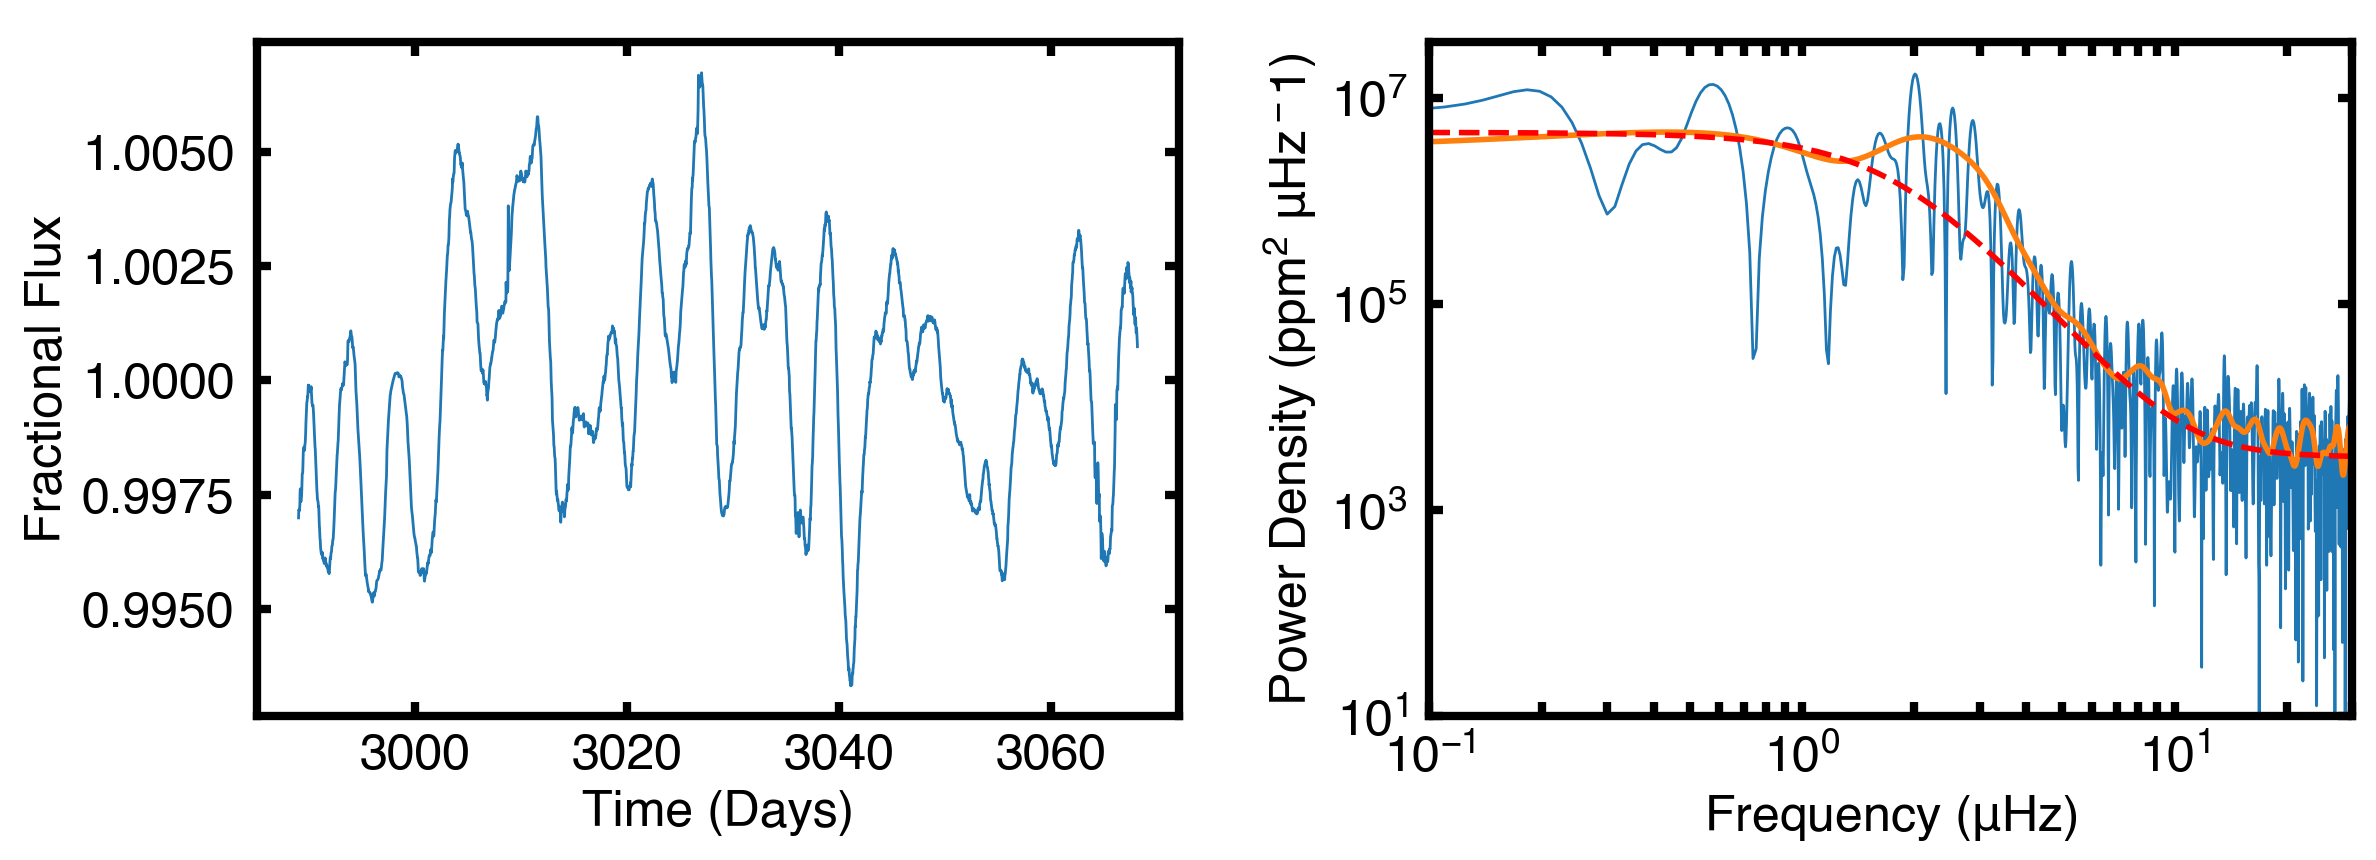
\includegraphics[width=\linewidth]{k2obs.png}
\caption{\ktwo lightcurve (left) and power spectrum (right) of Aldebaran. The red dashed line shows the background model, and the orange line is a heavily smoothed version of the power spectrum used to measure the frequency of maximum power. }
\label{fig:k2obs}
\end{center}
\end{figure}



%%%%%%%%%%%%%%%%%%%%%%%%%%%%%%%%%%%%%%%%%%%%%%%%%%%%%%%%%%%%%%%%%%%%%%%%%%%%%%%


%\bibliographystyle{mnras}
\bibliography{aldebaran.bib} 


%\begin{thebibliography}{10}
%\expandafter\ifx\csname url\endcsname\relax
%  \def\url#1{\texttt{#1}}\fi
%\expandafter\ifx\csname urlprefix\endcsname\relax\def\urlprefix{URL }\fi
%\providecommand{\bibinfo}[2]{#2}
%\providecommand{\eprint}[2][]{\url{#2}}
%
%\bibitem{TNaab2009}
%\bibinfo{author}{{Naab}, T.}, \bibinfo{author}{{Johansson}, P.~H.} \&
%  \bibinfo{author}{{Ostriker}, J.~P.}
%\newblock \bibinfo{title}{{Minor Mergers and the Size Evolution of Elliptical
%  Galaxies}}.
%\newblock \emph{\bibinfo{journal}{\apjl}} \textbf{\bibinfo{volume}{699}},
%  \bibinfo{pages}{L178--L182} (\bibinfo{year}{2009}).
%
%\end{thebibliography}

%%%%%%%%%%%%%%%%%%%%%%%%%%%%%%%%%%%%%%%%%%%%%%%%%%%%%%%%%%%%%%%%%%%%%%%%%%%%%%%


%%%%%%%%%%%%%%%%%%%%%%%%%%%%%%%%%%%%%%%%%%%%%%%%%%%%%%%%%%%%%%%%%%%%%%%%%%%%%%%


\end{document}
